\chapter*{\centering{\large{LEMBAR PERNYATAAN}}}
\onehalfspacing{}

Saya menyatakan dengan sesungguhnya bahwa skripsi dengan judul
\textbf{"Pendeteksian Keliling Luka Menggunakan Metode 
Border Following dengan Bantuan Interpolasi Spline"} yang disusun sebagai syarat untuk memperoleh gelar Sarjana Komputer
dari Program Studi Ilmu Komputer Universitas Negeri Jakarta adalah karya ilmiah
saya dengan arahan dari dosen pembimbing.

Sumber informasi yang diperoleh dari peneliti lain yang telah dipublikasikan 
yang disebutkan dalam teks Skripsi ini, telah dicantumkan dalam Daftar Pustaka 
sesuai dengan norma, kaidah dan etika penulisan ilmiah.

Jika dikemudian hari ditemukan sebagian besar skripsi ini bukan hasil karya saya 
sendiri dalam bagian-bagian tertentu, saya bersedia menerima sanksi pencabutan 
gelar akademik yang saya sanding dan sanksi-sanksi lainnya sesuai dengan 
peraturan perundang-undangan yang berlaku.

\vspace{4cm}

\begin{tabular}{p{7.5cm}c}
	&Jakarta, 26 Juli 2024\\
	&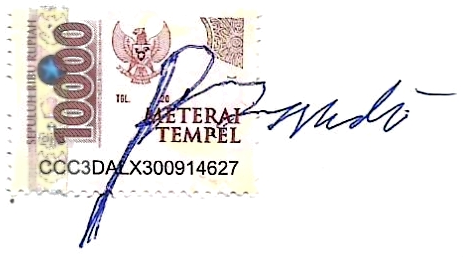
\includegraphics[keepaspectratio, width=5.533864542cm]
	{gambar/TTD_Pramudio_with_Materai.png}\\
	&Pramudio
\end{tabular}